As a reference we use 2010 analysis cut based approach documented
in~\ref{blah}. Table~\ref{tab:cutanalysis} summarizes selection
requirements re-tuned for this analysis.

\begin{table}[!ht]
  \begin{center}
 {\small
  \begin{tabular} {|c|c|c|c|c|c|}
  \hline
  Mass   &  $\pt^{\rm leading}$ & $\pt^{\rm trailing}$ & $\Delta\phi$ & $m_{ll}$ & $M_T$ \\ 
  \hline
  \hline
  H$_{120}$ & 20 & 10 & 2.0 & 40 & [70,120]\\
  H$_{130}$ & 25 & 10 & 1.5 & 45 & [75,125]\\
  H$_{140}$ & 25 & 15 & 1.5 & 45 & [80,130]\\
  H$_{150}$ & 27 & 25 & 1.5 & 50 & [80,150]\\
  H$_{160}$ & 30 & 25 & 1.0 & 50 & [90,160]\\
  \hline


 \hline
  \end{tabular}
  }
  \caption{Final Event selection requirements for a cut-based analysis}
   \label{tab:cutanalysis}
  \end{center}
\end{table}


\begin{table}[!ht]
  \begin{center}
 {\small
  \begin{tabular} {|c|c|c|c|}
  \hline
  Mass   &  R(2020) & R(2010) & R(new) \\
  \hline
  \hline
  H$_{120}$ & 7.6 & 5.0 & 3.4 \\
  H$_{130}$ & 2.7 & 2.3 & 1.7 \\
  H$_{140}$ & 1.4 & 1.4 & 1.2 \\
  H$_{150}$ & 0.88 & 0.93 & 0.80 \\
  H$_{160}$ & 0.44 & 0.60 & 0.43 \\
  \hline


 \hline
  \end{tabular}
  }
  \caption{Cut based analysis performance for different tunes. R(2020) refers 
  to 2010 analysis with minimum lepton \pt\ of 20 GeV. R(2010) is the same set of cuts,
  but the trailing lepton \pt\ is lowered to 10 GeV for Higgs mass hypothesis 
  of 160 GeV and lower. R(new) is a new set of cuts used in this analysis.}
   \label{tab:cutanalysis_perf}
  \end{center}
\end{table}


\begin{figure}[!htbp]
\begin{center}
   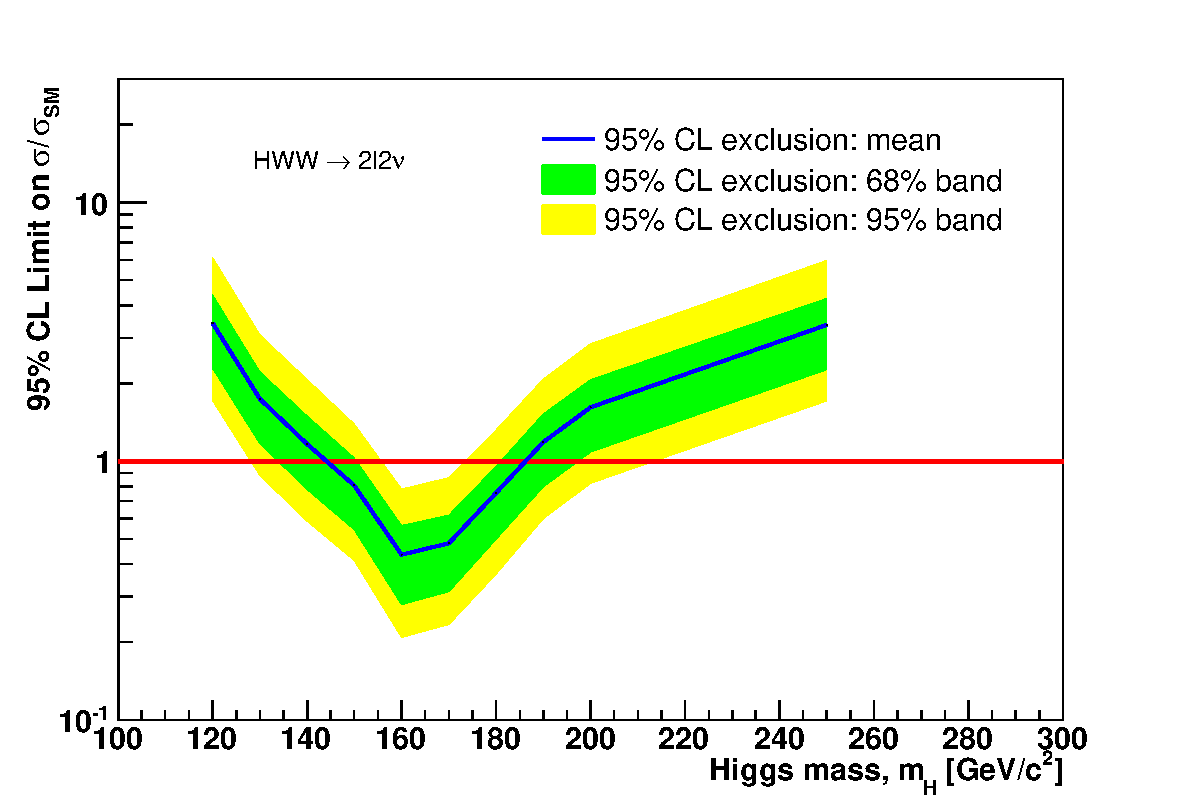
\includegraphics[width=0.9\textwidth]{figures/cut_based_limits.pdf}
   \caption{Cut based analysis expected upper limits at 95\%C.L. for 1\ifb\ of data.}
   \label{fig:cutbase_uls}
\end{center}
\end{figure}
